\documentclass{standalone}

\usepackage{tikz}
\usepackage{xcolor}
\usepackage{amsmath}
\usepackage{nicefrac}

\definecolor{jet}{HTML}{363636}
\definecolor{outerspace}{HTML}{464646}
\definecolor{granitegray}{HTML}{616161}
\definecolor{raisinblack}{HTML}{252525}
\definecolor{tigerseye}{HTML}{EB9438}
\definecolor{denimblue}{HTML}{2B3EAB}
\definecolor{englishgreen}{HTML}{26523C}
\definecolor{upmaroon}{HTML}{780D14}
\definecolor{isabelline}{HTML}{EDEDED}
\definecolor{palmleaf}{HTML}{6DA63F}

\usetikzlibrary{shapes.arrows,chains}
\newcommand{\I}{\color{isabelline}}
\newcommand{\N}{{\color{tigerseye} n}\I}
% \newcommand{\C}{\color{granitegray}}
\newcommand{\C}{\color{palmleaf}}

\begin{document}

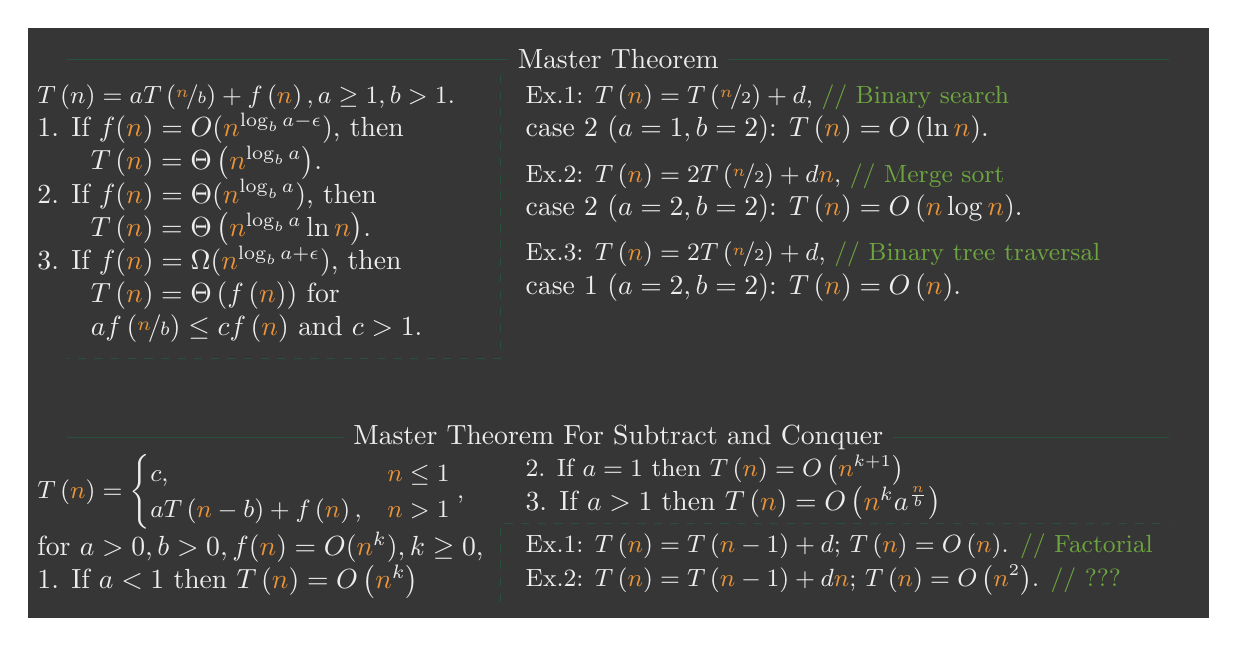
\begin{tikzpicture}
  % Background
  \fill [jet] (0, -2.5) rectangle (15, 5);

  % Block name
  \node at(7.5, 4.6) (mastermethod) {\I Master Theorem};
  \draw[englishgreen] (0.5,4.6) -- (mastermethod.west); 
  \draw[englishgreen] (mastermethod.east) -- (14.5, 4.6);

  \node[align=left] at(0, 4.4)[anchor=north west] {
    \small
    $\I T\left(n\right)=aT\left(\nicefrac{\N}{b}\right) + f\left(\N\right), a \ge 1, b > 1.$\\
    \I 1. If $f(\N)=O(\N^{\log_{b} a - \epsilon})$, then \\
    \I \hspace{5.6mm} $T\left(\N\right) = \Theta\left(\N^{\log_{b} a}\right)$.\\
    \I 2. If $f(\N)=\Theta(\N^{\log_{b} a})$, then \\
    \I \hspace{5.6mm} $T\left(\N\right) = \Theta\left(\N^{\log_{b} a}\ln \N\right)$.\\
    \I 3. If $f(\N)=\Omega(\N^{\log_{b} a + \epsilon})$, then \\
    \I \hspace{5.6mm} $T\left(\N\right) = \Theta\left(f\left(\N\right)\right)$ for\\
    \I \hspace{5.6mm} $af\left(\nicefrac{\N}{b}\right) \le cf\left(\N\right)$ and $c>1$.\\
  };

  \draw[englishgreen,dashed] (6, 4.4) -- (6,0.8) -- (0.5, 0.8); 

  \node[align=left] at(6.2, 4.4)[anchor=north west] {
    \small \I Ex.1:
    \I $T\left(\N \right)=T\left(\nicefrac{\N}{2}\right) + d$,  \C // Binary search \\
    \I case 2 $(a=1,b=2)$: $T\left(\N\right)=O\left(\ln\N\right)$.
  };

  \node[align=left] at(6.2, 3.4)[anchor=north west] {
    \small \I Ex.2:
    \I $T\left(\N \right)=2T\left(\nicefrac{\N}{2}\right) + d\N$, \C // Merge sort\\
    \I case 2 $(a=2,b=2)$: $T\left(\N\right)=O\left(\N\log\N\right)$. 
  };

  \node[align=left] at(6.2, 2.4)[anchor=north west] {
    \small \I Ex.3:
    \I $T\left(\N \right)=2T\left(\nicefrac{\N}{2}\right) + d$,  \C // Binary tree traversal\\
    \I case 1 $(a=2,b=2)$: $T\left(\N\right)=O\left(\N\right)$.
  };

  % Block name
  \node at(7.5, -0.2) (mastermethod) {\I Master Theorem For Subtract and Conquer};
  \draw[englishgreen] (0.5,-0.2) -- (mastermethod.west); 
  \draw[englishgreen] (mastermethod.east) -- (14.5,-0.2);

  \node[align=left] at(0,-0.3)[anchor=north west] {
    \small
    $\I T\left(\N \right)=
        \begin{cases}
          c,& \N \le 1 \\
          aT\left(\N - b\right) + f\left(\N\right),& \N > 1
        \end{cases},$\\
     \I for $a > 0, b > 0, f(\N) = O(\N^{k}), k \ge 0$,\\
     \I 1. If $a<1$ then $T\left(\N\right) = O\left(\N^{k}\right)$
  };

  \node[align=left] at(6.2,-0.3)[anchor=north west] {
    \small
     \I 2. If $a=1$ then $T\left(\N\right) = O\left(\N^{k + 1}\right)$\\
     \I 3. If $a>1$ then $T\left(\N\right) = O\left(\N^{k}a^{\frac{\N}{b}}\right)$
  };

  \node[align=left] at(6.2, -1.3)[anchor=north west] {
    \small \I Ex.1:
    \I $T\left(\N \right)=T\left(\N - 1\right) + d$; $\I T\left(\N\right)=O\left(\N\right)$. \C// Factorial
  };

  \node[align=left] at(6.2, -1.7)[anchor=north west] {
    \small \I Ex.2:
    \I $T\left(\N \right)=T\left(\N - 1\right) + d\N$; $\I T\left(\N\right)=O\left(\N^{2}\right)$. \C// ???
  };

  \draw[englishgreen,dashed] (6, -2.3) -- (6,-1.3) -- (14.5,-1.3); 
\end{tikzpicture}

\end{document}
